\documentclass[12pt]{book}
%\usepackage[papersize={125mm,205mm},tmargin=1.5cm,bmargin=1.5cm,hmargin=1cm]{geometry}
\usepackage[utf8x]{inputenc}
\usepackage{../../latex/preambule_NSI_2022/MichaelNSI2022}



\setcounter{minitocdepth}{2}
\usepackage{qrcode}

\mtcselectlanguage{francais}


%%%%%%%% Faire de l'air autour d'une fraction (surtout ds un tableau)
\newcommand{\delair}[1]{\ensuremath\displaystyle\psframebox[framesep=0.15em,linestyle=none]{ \displaystyle#1}}


\fancyhead[L]{\includegraphics[scale=0.03]{../../latex/preambule_NSI_2022/LATEXimages/NSI_600}\normalsize N.S.I : Numérique et Science Informatique}
\fancyhead[R]{\normalsize Terminale}
\renewcommand\headrulewidth{1pt}
\renewcommand\footrulewidth{1pt}
%\fancyfoot[L]{Terminale $S$}
\fancyfoot[C]{\includegraphics[scale=0.75]{../../latex/preambule_NSI_2022/creative_licence_compact}}%\textbf{Page \thepage/\pageref{LastPage}}}
%\fancyfoot[R]{\textbf{Page \thepage}}%\pageref{LastPage}}}


\fancyfoot[LE]{$\blacksquare$\,$\blacksquare$\;\thepage}%
\fancyfoot[RO]{\thepage\;$\blacksquare$\,$\blacksquare$}%
\fancyfoot[LO]{\uppercase{\sffamily{Devoir \thechapter}}}
\fancyfoot[RE]{\normalsize\sffamily Devoir \thechapter }
\pagestyle{fancy}

\renewcommand{\arraystretch}{1} 
\renewcommand*\tabularxcolumn[1]{>{\centering\arraybackslash}m{#1}}
%\usepackage[bloc,completemulti]{automultiplechoice}  

\usepackage{microtype} %ameliorations typographiques

\usepackage{comment}
%\affichecorrectionfalse
%\affichecorrectiontrue
%\affichepreuvefalse
%\excludecomment{preuve}

\lstnewenvironment{sql}[1][]{ 
\lstset{
upquote=true,
columns=flexible,
basicstyle=\ttfamily,
language={SQL},
commentstyle=\color{gray},
xleftmargin=2em, %espace a gauche
xrightmargin=2em, %espace a droite
aboveskip=\topsep, %espace au-dessus
belowskip=\topsep, %espace en-dessous
#1
}
}{}

\usepackage{tcolorbox}



%\usepackage{picins}
\usepackage[tikz]{bclogo}
\author{M.Meyroneinc}
\title{Terminale}

\begin{document}


	\setcounter{chapter}{6}

\bilan	
\theme{T9}
%\Tneuf

\chapter{Bac Blanc}

\vspace{0,25cm}

Ce sujet, noté sur 20, comporte deux exercices notés respectivement sur 8 et 12 points. 
Les deux exercices sont à traiter en intégralité. Ce sujet n’est pas à rendre avec votre copie.\\
Lors de la correction, la plus grande attention sera portée à la clarté de vos réponses.\\ Le fait de répondre sans faire de phrases sera sanctionné.   Lorsque vous écrirez du code, pensez à bien marquer de manière visible les indentations éventuelles.


\medskip
\bigskip

\textbf{\textsc{Exercice 1} \quad 8 points\hfill Thèmes : SQL}

\bigskip

L’énoncé de cet exercice utilise la convention suivante : les clés primaires seront soulignées et les clés étrangères seront précédées d’un $\#$.  

Le satellite GAIA a pour mission de cartographier un très grand nombre d’objets autour du Système Solaire. Régulièrement un catalogue est produit
pour publier les données obtenues. Il est disponible sous différents formats dont par exemple sous forme de fichier csv.  

N\_Obj identifie chaque objet cartographié de manière unique. 

Voici un extrait du catalogue :


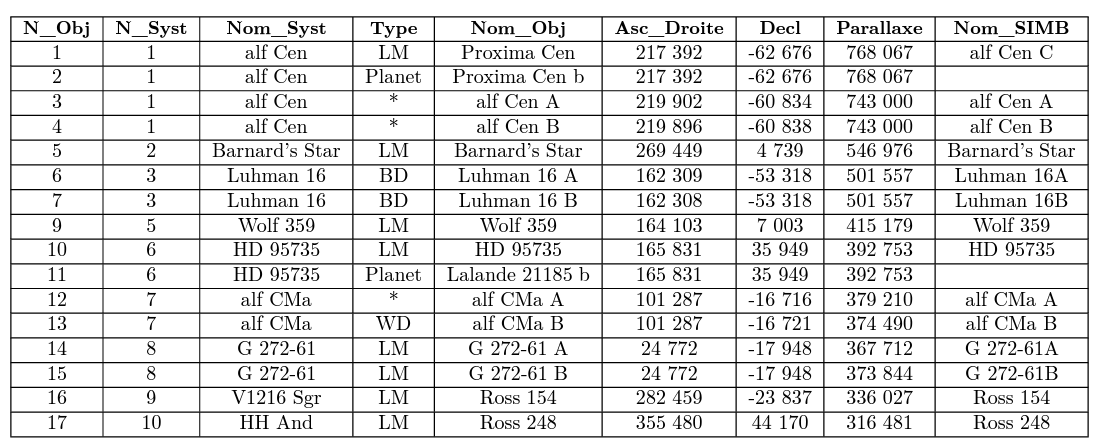
\includegraphics[scale=0.45]{data/bacblancsql.png} 

Pour manipuler plus facilement les données, un chercheur utilise un système de base de données relationnelle, dans lequel il crée le schéma relationnel de la table Gaia :  

\begin{sql}
 Gaia(N_Obj : Int, N_Syst : Int, Nom_Syst : String, #Type : String , Nom_Obj : String,   Asc_Droite : Real, Decl : Real, Parallaxe : Real, Nom_SIMB : String)  
\end{sql}

\newpage

\textbf{Partie A : Schéma relationnel}

\begin{enumerate}
\item Justifier pourquoi l’attribut N\_Obj a été choisi comme clé primaire de la table Gaia.\\ 
Le type de l’objet (attribut {\tt Type}) n’est pas une information directement compréhensible et le chercheur décide de créer une nouvelle table appelée {\tt Typologie}.\\
La clé primaire est {\tt Type}.

Soit la table {\tt Typologie} contenant les informations suivantes : 

	\begin{center}
			{\footnotesize \begin{tabular}{|c|c|}
					\hline
					Type      & Libelle\_Type \\
					\hline
					LM   & Etoile de faible masse     \\
					\hline
					Planet & Planète       \\
					\hline
					*   & Etoile   \\
					\hline
					BD & Naine Brune       \\
					\hline
					WD & Naine Blanche      \\
					\hline
				\end{tabular}} \end{center}

\item Proposer le schéma relationnel de la table {\tt Typologie}.
\item Parmi les 4 commandes suivantes, une seule ne provoque pas d’erreur. Pour chacune de ces commandes, indiquer si elle provoque une erreur ou pas. En cas d’erreur, expliquer la cause de cette erreur.
\begin{enumerate}
\item .\\
\begin{sql}
INSERT INTO Gaia VALUES ('8', 4, 'WISEA J085510', 'Naine Brune', 'WISEA J085510', 133.781,-7.244, 439.000, 'WISEA J085510') ;
\end{sql}

\item .\\
\begin{sql}
INSERT INTO Gaia VALUES (9, 4, 'WISEA J085510', 'Naine Brune', 'WISEA J085510', 133.781,-7.244, 439.000, 'WISEA J085510') ;
\end{sql} 

\item .\\
\begin{sql}
INSERT INTO Gaia VALUES (8, 4, 'WISEA J085510', 'Naine Brune', 'WISEA J085510', 133.781,-7.244, 439.000, 'WISEA J085510') ; 
\end{sql}

\item .\\
\begin{sql}
INSERT INTO Gaia VALUES (8, 4, 'WISEA J085510', 'Naine Brune', 'WISEA J085510', '133.781',-7.244, 439.000, 'WISEA J085510') ;
\end{sql}

	\end{enumerate}
\item Expliquer pourquoi le code SQL suivant ne fonctionne pas : 
\begin{sql}
INSERT INTO Typologie VALUES (BD, Trou Noir) ;
\end{sql}
\item Indiquer le résultat de la requête suivante exécutée sur l’extrait présenté : 
\begin{sql}
SELECT N_Obj, Parallaxe 
FROM Gaia 
WHERE Type = Planet;
\end{sql}
\item Écrire la requête qui permet de récupérer le nom du système, le nom de l’objet et le libellé du type pour des objets ayant une parallaxe supérieure à 400 000 et étant des ’Etoile de faible masse’. La requête proposée utilisera obligatoirement une jointure.
\end{enumerate}

\bigskip


\textbf{\textsc{Exercice 2} \quad 7 points\hfill Thème : Probabilités}

\medskip

Une urne contient des jetons blancs et noirs tous indiscernables au toucher.

Une partie consiste à prélever au hasard successivement et avec remise deux jetons de cette urne.

On établit la règle de jeu suivante:

\setlength\parindent{1cm}
\begin{itemize}
\item[$\bullet~~$] un joueur perd 9 euros si les deux jetons tirés sont de couleur blanche ;
\item[$\bullet~~$] un joueur perd 1 euro si les deux jetons tirés sont de couleur noire ;
\item[$\bullet~~$] un joueur gagne 5 euros si les deux jetons tirés sont de couleurs différentes.
\end{itemize}
\setlength\parindent{0cm}

\medskip

\begin{enumerate}
\item On considère que l'urne contient 2 jetons noirs et 3 jetons blancs.
	\begin{enumerate}
		\item Modéliser la situation à l'aide d'un arbre pondéré.
		\item Calculer la probabilité de perdre $9$ \euro{} sur une partie.
	\end{enumerate}	
\item On considère maintenant que l'urne contient 3 jetons blancs et au moins deux jetons noirs mais on ne connait pas le nombre exact de jetons noirs. On appellera $N$ le nombre de jetons noirs.
	\begin{enumerate}
		\item Soit $X$ la variable aléatoire donnant le gain du jeu pour une partie.
		
Déterminer la loi de probabilité de cette variable aléatoire.
		\item Résoudre l'inéquation pour $x$ réel:
		
\[-x^2  + 30x - 81 > 0\]

		\item En utilisant le résultat de la question précédente, déterminer le nombre de jetons noirs que l'urne doit contenir afin que ce jeu soit favorable au joueur.
		\item Combien de jetons noirs le joueur doit-il demander afin d'obtenir un gain moyen maximal ?
	\end{enumerate}
\item On observe $10$ joueurs qui tentent leur chance en effectuant une partie de ce jeu, indépendamment les uns des autres. On suppose que 7 jetons noirs ont été placés dans l'urne (avec 3 jetons blancs). 

Quelle est la probabilité d'avoir au moins $1$ joueur gagnant $5$ euros?
\end{enumerate}


\textbf{\textsc{Exercice 3} \hfill 7 points}

\medskip

\emph{Principaux domaines abordés}: Probabilités conditionnelles et indépendance. Variables aléatoires.

\medskip

Lors d'une kermesse, un organisateur de jeux dispose, d'une part, d'une roue comportant quatre cases blanches et huit cases rouges et, d'autre part, d'un sac contenant cinq jetons portant les numéros 1, 2, 3, 4 et 5.

Le jeu consiste à faire tourner la roue, chaque case ayant la même probabilité d'être obtenue, puis à extraire un ou deux jetons du sac selon la règle suivante :

\setlength\parindent{1cm}
\begin{itemize}
\item[$\bullet~~$] si la case obtenue par la roue est blanche, alors le joueur extrait un jeton du sac ;
\item[$\bullet~~$] si la case obtenue par la roue est rouge, alors le joueur extrait successivement et sans remise deux jetons du sac.
\end{itemize}
\setlength\parindent{0cm}

Le joueur gagne si le ou les jetons tirés portent tous un numéro impair.

\medskip

\begin{enumerate}
\item Un joueur fait une partie et on note $B$ l'évènement \og la case obtenue est blanche \fg,
$R$ l'évènement \og la case obtenue est rouge\fg{} et $G$ l'évènement \og le joueur gagne la partie \fg. 
	\begin{enumerate}
		\item Donner la valeur de la probabilité conditionnelle $P_B(G)$.
		\item On admettra que la probabilité de tirer successivement et sans remise deux jetons impairs est égale à $0,3$. 
		
Recopier et compléter l'arbre de probabilité suivant:


	\end{enumerate}

\item
	\begin{enumerate}
		\item Montrer que $P(G) = 0,4$.
		\item Un joueur gagne la partie.
		
Quelle est la probabilité qu'il ait obtenu une case blanche en lançant la roue?
	\end{enumerate}
\item Les évènements $B$ et $G$ sont-ils indépendants ? Justifier.
\item Un même joueur fait dix parties. Les jetons tirés sont remis dans le sac après chaque partie.

On note $X$ la variable aléatoire égale au nombre de parties gagnées.
	\begin{enumerate}
		\item Expliquer pourquoi $X$ suit une loi binomiale et préciser ses paramètres.
		\item Calculer la probabilité, arrondie à $10^{-3}$ près, que le joueur gagne exactement trois parties sur les dix parties jouées.
		\item Calculer $P (X \geqslant 4)$ arrondie à $10^{-3}$ près.
		
Donner une interprétation du résultat obtenu.
	\end{enumerate}
\item Un joueur fait $n$ parties et on note $p_n$ la probabilité de l'évènement \og le joueur gagne au moins une partie \fg.
	\begin{enumerate}
		\item Montrer que $p_n = 1 - 0,6^n$.
		\item Déterminer la plus petite valeur de l'entier $n$ pour laquelle la probabilité de gagner au moins une partie est supérieure ou égale à $0,99$.
	\end{enumerate}
\end{enumerate}

\bigskip






\end{document}